\subsection{Элементы орбиты}
Вектором состояния X назовем упорядоченную совокупность переменных, полностью определяющих состояние системы в заданный момент времени.
В простейшем случае такой набор состоит из положения $\mathbf{r}$ и скорости $\mathbf{v}$ материальной точки. 
Также в этот набор могут входить площадь поверхности и другие параметры космического объекта, оказывающие влияние на его движение.

Однако, в ходе орбитального движения $\mathbf{r}$ и $\mathbf{v}$ меняются за виток значительно, что приводит к снижению точности при численном интегрировании.
Поэтому зачастую в ходе решения задачи двух тел в небесной механике используют не радиус-вектор и скорость, а элементы орбиты.
Самыми распространенными из них являются кеплеровы элементы и модифицированные равнодественные элементы (MEE).
В элементах орбиты быстро меняющаяся переменная, описывающая положение КО на орбите, отделена от медленно меняющихся переменных,
определяющих ориентацию и форму орбитальной плоскости.
\begin{center}
    \begin{minipage}[t]{0.45\textwidth}
        \vspace{0pt}
        \textbf{Кеплеровы элементы:}
        \begin{itemize}
            \item наклонение $i$
            \item долгота восходящего узла $\Omega$
            \item аргумент перицентра $\omega$
            \item эксцентриситет $e$
            \item большая полуось $a$
            \item истинная аномалия $\nu$
        \end{itemize}
    \end{minipage}
    \hspace{1cm}
    \begin{minipage}[t]{0.45\textwidth}
        \vspace{0pt}
        \textbf{MEE:}
        \begin{itemize}
            \item $a = a$
            \item $h = e \sin\left(\omega + I \Omega \right)$
            \item $k = e \cos\left(\omega + I \Omega \right)$
            \item $p = \left[\tan{\frac{i}{2}}\right]^I \sin(\Omega)$
            \item $q = \left[\tan{\frac{i}{2}}\right]^I \cos(\Omega)$
            \item $\lambda = M + \omega + I \Omega$
        \end{itemize}
    \end{minipage}
\end{center}

\begin{figure}[h!]
    \centering
    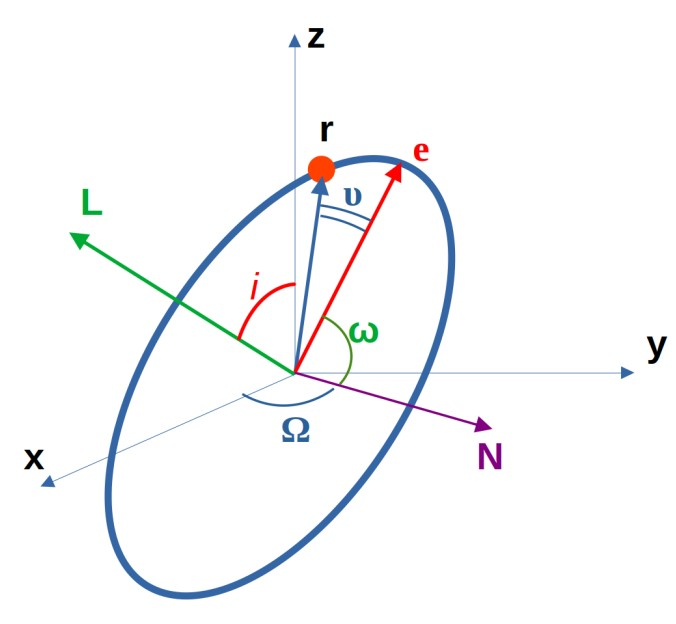
\includegraphics[width=0.6\linewidth]{../images/review/kepler.jpg}
    \captionof{figure}{Кеплеровы элементы орбиты. Центр декартовых координат привязан к центру масс Земли. Ось $Ox$ направлена в точку весеннего равноденствия, 
    ось $Oz$ -- нормаль к плоскости эклиптики, 
    ось $Oy$ дополняет до правой тройки.
    $\mathbf{N}$ лежит на линии пересечения плоскости эклиптики с плоскостью орбиты.
    $\mathbf{L}$ -- момент импульса КО,направлен по нормали к орбитальной плоскости. 
    $\mathbf{e}$ равен по модулю эксцентриситету и направлен на перицентр.}
    \label{fig:kepler}
\end{figure}

Кеплеровы элементы удобны для визуальной интерпретации орбиты (рис. \ref{fig:kepler}).
Первые 3 переменные задают ориентацию орбитальной плоскости в инерциальной системе координат,
эксцентриситет и большая полуось фиксируют форму и размеры эллипса, а истинная аномалия определяет положение КО на орбите.
В качестве последней переменной также могут использоваться эксцентрическая аномалия $E$ и средняя аномалия $M$.
Удобство использования средней аномалии заключается в том, что она меняется со временем равномерно.
Недостаток кеплеровых элементов -- вырожденность при $i = 0$, $i = \pi$ и $e = 0$.
Как следствие, они плохо подходят для интегрирования.

Чтобы избавиться от вырожденности, вводится другой набор элементов -- модифицированные равноденственные элементы.
В MEE величина I может принимать два значения:
\[
I = \left\{
\begin{array}{ll}
+1, & \text{если } i < \pi / 2, \\
-1, & \text{если } i \ge \pi / 2
\end{array}
\right.
\]

Также в MEE применяется эксцентрическая долгота $F$ и истинная долгота $L$. 
Они выражаются через кеплеровы элементы следующим образом:
\begin{align*}
    F &= E + \omega + I \Omega \\
    L &= \nu + \omega + I \Omega
\end{align*}

\subsection{Прогноз траектории космического объекта}
Задача прогнозирования движения -- по начальному вектору состояния $\mathbf{x_0}$ определить траекторию $\mathbf{x}(t)$ объекта.
В основе описания динамики космических аппаратов лежит 2 закон Ньютона, 
поэтому расчет траектории сводится к решению задачи Коши для ОДУ вида:
\begin{equation}
    \begin{cases}
        \dot{\mathbf{x}} = f(\mathbf{x}, t), \\
        \mathbf{x} \big|_{t = t_0} = \mathbf{x_0}
        \label{eq:prognoz_task}
    \end{cases}
\end{equation}

При расчете траектории применяются несколько существенно разных подходов. 
Первый из них, аналитический, использует основные факторы, определяющие эволюцию орбиты.
Характерной особенностью аналитических вычислений является низкая ресурсоемкость и невысокая точность.
Таким образом, аналитика обладает высокой качественной предсказательной способностью на коротких временных интервалах, 
«схватывая» главные тренды изменения орбиты.

Численные методы, напротив, позволяют учесть произвольное число сложных возмущающих факторов.
Однако прецизионный численный расчет требует значительно больше вычислений. 
Это связано с ресурсоемкостью расчета правой части ОДУ и,
соответственно, с выбором шага интегрирования для обеспечения заданной точности.

Компромиссом являются полуаналитические подходы, 
в которых используется комбинация численных и аналитических расчетов.
Полуаналитические модели учитывают широкий спектр возмущающих воздействий, 
что позволяет эффективно производить вычисления без потери точности.

Далее приведен краткий обзор основных подходов к прогнозу траектории.

\subsubsection{Аналитический прогноз}
Рассмотрим возмущенную задачу двух тел:

\begin{equation}
    \ddot{\mathbf{r}} = - \frac{\mu \mathbf{r}}{r^3} + \mathbf{f},
    \label{eq:analyt_rv}
\end{equation}
где $\mu$ -- гравитационный параметр Земли, $\mathbf{f}$ -- возмущающее ускорение, которое может быть разложено по орбитальной СК на радиальную, тангенциальную и нормальную компоненты:

\begin{equation*}
    \mathbf{f} = R \mathbf{e}_r + T \mathbf{e}_t + N \mathbf{e}_n,
\end{equation*}
\begin{align*}
    \mathbf{e}_r &= \mathbf{r} / |r| \\
    \mathbf{e}_n &= \mathbf{r} \times \mathbf{v} / |\mathbf{r} \times \mathbf{v}| \\
    \mathbf{e}_t &= \mathbf{e_n} \times \mathbf{e_r}
\end{align*}

\begin{figure}[h!]
    \centering
    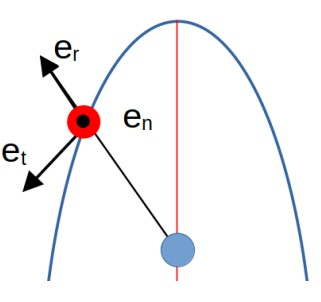
\includegraphics[width=0.4\linewidth]{../images/review/orbital_system.jpg}
    \captionof{figure}{Орбитальная система}
    \label{fig:orbital_system}
\end{figure}

% Byron, p. 485-486
Преобразуем систему ОДУ (\ref{eq:analyt_rv}) для перехода к кеплеровым элементам.
% \begin{align*}
%     & \frac{da}{dt} = \frac{2 a e^2}{h} \sin(\nu) R 
%                     + \frac{2 a^2 h}{\mu r} T \\
%     & \frac{de}{dt} = \frac{h}{\mu} \left[ \sin(\nu) R +
%                      (e + 2 \cos(\nu) + e \cos^2(\nu)) / (1 + e cos \nu) T \right] \\
%     & \frac{di}{dt} = \frac{r}{h} \cos(\omega + \nu) N \\
%     & \frac{d \Omega}{dt} = \frac{r \sin(\omega + \nu) N}{h \sin(i)} \\
%     & \frac{d \omega}{dt} = - \frac{h}{\mu e} \cos(\nu) R 
%                             - \frac{r}{h} \ctg(i) \sin(\omega + \nu) n
%                             + \frac{(h^2 + r \mu) \sin(\nu)}{\mu e h} T \\
%     & \frac{dM}{dt} = n - \frac{1}{na}\left(\frac{2r}{a} - \frac{1 - e^2}{e} \cos(\nu)\right) R
%                         - \frac{1 - e^2}{nae} \left(1 + \frac{r}{p}\right) sin(\nu) T
% \end{align*}
Если возмущающая сила является потенциальной: $\mathbf{f} = \nabla R$, то система примет вид:

\begin{align*}
    & \frac{da}{dt} = \frac{2}{na} \frac{\partial R}{\partial M} \\
    & \frac{de}{dt} = \frac{(1 - e^2)^{1 / 2}}{n a^2 e^2}
                    \left((1 - e^2)^{1 / 2} \frac{\partial R}{\partial M} 
                    - \frac{\partial R}{\partial \omega} \right) \\
    & \frac{di}{dt} = \frac{1}{h \sin(i)} \left(cos(i) \frac{\partial R}{\partial \omega} 
                                                        - \frac{\partial R}{\partial \omega} \right) \\
    & \frac{d \Omega}{dt} = \frac{1}{h \sin(i)} \frac{\partial R}{\partial i} \\
    & \frac{d \omega}{dt} = - \frac{\cos(i)}{h \sin(i)} \frac{\partial R}{\partial i}
                            + \frac{(1 - e^2)^{1 / 2}}{n a^2 e^2} \frac{\partial R}{\partial e} \\
    & \frac{dM}{dt} = n - \frac{1 - e^2}{n a^2 e} \frac{\partial R}{\partial e} 
                        - \frac{2}{na} \frac{\partial R}{\partial a}
\end{align*}
где $n = \sqrt{\frac{\mu}{a^3}}$ -- среднее движение, $h = n a^2 (1 - e^2)^2$.

Для построения аналитического решения воспользуемся возмущающим потенциалом от второй гармоники:
 \begin{equation}
    R = - \frac{\mu J_2}{r} \left( \frac{R_\oplus}{r} \right)^2 
        \frac{3}{2} \left(\sin^2(\phi) - \frac{1}{3}\right),
 \end{equation}
где $\phi$ -- широта точки.

Подставив соотношение $sin(\phi) = sin(i) sin(\omega + \nu)$, получим, что $R$ может быть представлена в виде суммы:

\begin{align*}
    & R = R_s + R_p \\
    & R_s = - \frac{3 \mu J_2}{2 r} \left( \frac{R_\oplus}{r} \right)^2 
            \left( \frac{\sin^2(i)}{2} - \frac{1}{3} \right) \\
    & R_p = \frac{3 \mu J_2}{2 r} \left( \frac{R_\oplus}{r} \right)^2
            \frac{\sin^2(i) \cos(2(\omega + \nu))}{2}
\end{align*}

Видно, что первое слагаемое потенциала вызывает постоянное или так называемое вековое возмущение орбиты. 
Период таких возмущений значительно превышает орбитальный период. 
Короткопериодические возмущения, порождаемые слагаемым $R_p$, не приводят к изменениям орбиты на значительном промежутке времени.

Усреднив $R_s$ по периоду, получим:
\begin{equation*}
    R_{avg} =  - \frac{\mu J_2}{2 a} \left( \frac{R_\oplus}{r} \right)^2 
                \left( \frac{3}{4} \sin^2(i) - \frac{1}{2} \right)
                \left( \frac{1}{(1 - e^2)^{3/2}} \right)
\end{equation*}

Подстановка $R_{avg}$ в ОДУ дает вековые возмущения кеплеровых элементов орбиты

\begin{align*}
    & \dot{a}_{sec} = 0 \\
    & \dot{e}_{sec} = 0 \\
    & \dot{i}_{sec} = 0 \\
    & \dot{\Omega}_{sec} = - \frac{3 n R^{2}_\oplus J_2}{2 p^2} \cos(i) \\
    & \dot{\omega}_{sec} = \frac{3 n R^{2}_\oplus J_2}{4 p^2} (4 - 5 \sin^2(i)) \\
    & \dot{M_0}_{sec} = - \frac{3 n R^{2}_\oplus J_2 \sqrt{1 - e^2}}{4 p ^2}
                            (3 \sin^2(i) - 2)
\end{align*}

Аналогичным образом могут быть выделены короткопериодические возмущения. В частности:

\begin{equation*}
    \delta a = \gamma_3 a \left[ (3z \sin^2(\omega + \nu) - 1) \left(\frac{a}{r}\right)^3
                                    - \frac{3z - 2}{2 \eta^3}  \right],
\end{equation*}
где $\gamma_3 = -J_2 \left(\frac{R_\oplus}{a}\right)^2$, $\eta = \sqrt{1 - e^2}$, $z = \sin^2(i)$.

Так как большая полуось, эксцентриситет и наклонение не испытывают вековых возмущений, 
средние значения долготы восходящего узла и аргумента перицентра легко интегрируются аналитически:
\begin{align*}
    & \Omega(t) = \Omega_0 + \Omega_{sec} (t - t_0) \\
    & \omega(t) = \omega_0 + \omega_{sec} (t - t_0) \\
\end{align*}
Для получения выражения для $a$ необходимо провести процедуру усреднения среднего движения
\begin{equation*}
    a = \bar{a} + \delta a \rightarrow  \bar{a} = a_0 - \delta a_0
\end{equation*}
\begin{equation*}
    \bar{n} = \sqrt{\frac{\mu}{\bar{a}^3}}
\end{equation*}

В результате получим:
\begin{equation*}
    M(t) = M_0 + (\bar{n} + \dot{M_0}_{sec}) (t - t_0)
\end{equation*}

Более детальное решение задачи аналитического расчета траектории представлено в серии моделей SGP \cite{spacetrack80}.
Модели используют данные в формате TLE, предоставляемые американской службой NORAD. 
В TLE содержатся не только средние кеплеровы элементы орбиты, но и первая и вторая производные среднего движения.
Модели движения SGP аналитически учитывают возмущения от сжатия Земли, сопротивления атмосферы, гравитации Луны и Солнца.
Из-за сильного влияния атмосферного торможения ошибка прогноза на низких орбитах составляет порядка 1 километра в день.
Для средних и высоких орбит ошибка значительно меньше -- несколько сотен метров на недельном интервале \cite{vallado2008}. 

\subsubsection{Численно-аналитический прогноз}
Стимулом к развитию численно-аналитических методов послужил быстрый рост количества
объектов в околоземном пространстве и необходимость их непрерывного отслеживания и каталогизации.
Для таких задач аналитические методы не удовлетворяют требуемой точности, а численные методы
не подходят в силу высокой ресурсоемкости. Численно-аналитические методы, в свою очередь,
объединяют точность и быстродействие за счет гибкой настройки модели движения.

В основе численно-аналитических моделей лежит разделение возмущений на вековые, 
короткопериодические и долгопериодические.
На начальном этапе происходит усреднение орбитальных элементов, 
чтобы исключить высокочастотные возмущения орбиты. Эта операция позволяет в дальнейшем
интегрировать медленно меняющиеся средние элементы с большим шагом (порядка половины дня).
На заключительном этапе прогноза мгновенные значения элементов орбиты вычисляются аналитически по средним элементам.

Частным случаем численно--аналитических методов является модель DSST \cite{danielson1995}, разработанная для
системы контроля околоземного пространства Европейского космического агентства (SSA).
Математическая модель DSST опирается на методы усреднения и вариации параметров.

Усредненные уравнения движения для консервативной возмущающей силы с потенциалом $R$:

\begin{equation*}
    \frac{d\bar{c}_i}{dt} = -\sum_{j=1}^{6} \left\{\bar{c}_i, \bar{c}_j \right\} 
                                \frac{\partial \bar{R}}{\partial\bar{c}_j} \qquad i=1 \dots 5
\end{equation*}

При наличии неконсервативной силы правая часть дополнительно усредняется по витку:

\begin{equation*}
    \frac{d\bar{c}_i}{dt} = \frac{1}{2 \pi} \int_{0}^{2 \pi} \frac{\partial\bar{c}_i}{\partial\dot{\mathbf{r}}} 
                        \cdot \mathbf{Q} d\lambda \qquad i=1 \dots 5
\end{equation*}

Выражение для быстроменяющейся средней долготы:

\begin{equation*}
    \frac{d \bar{\lambda}}{dt} = \frac{d\bar{c}_6}{dt} = 
        \bar{n} -\sum_{j=1}^{6} \left\{\bar{c}_6, \bar{c}_j \right\} 
                                \frac{\partial \bar{R}}{\partial\bar{c}_j}
                +\frac{1}{2 \pi} \int_{0}^{2 \pi} \frac{\partial\bar{c}_6}{\partial\dot{\mathbf{r}}} 
                        \cdot \mathbf{Q} d\lambda
\end{equation*}

Переход к мгновенным элементам:

\begin{equation*}
    c_i = \bar{c}_i + \sum_{j=1}^{N} e^j \eta_{i, j}\left(\bar{a}, \bar{\lambda}\right) \qquad i = 1 \dots 6
\end{equation*}

В последних уравнениях были введены следующие обозначения:
\begin{align*}
    \bar{c}_{i=1 \dots 6} &: \text{средние равноденственные элементы} \left[\bar{h}, \bar{k}, \bar{k}, \bar{p}, \bar{q}, \bar{\lambda}\right] \\
    \bar{R} &: \text{усредненный возмущающий потенциал для консервативной силы} \\
    \mathbf{Q} &: \text{неконсервативная сила} \\
    \bar{n} &: \text{усредненное среднее движение} \\
    \left\{\bar{c}_i, \bar{c}_j \right\} &: \text{скобки Пуассона} \\
    \eta_{i, j} &: 2\pi \text{-периодические функции}
\end{align*}

Точность прогноза по модели DSST отличается для разных классов орбит \cite{setty2016}.
Среднеквадратичное отклонение при сравнении с численным расчетом на 7 суток составляет от 10 метров для НОО до 20 метров для ГСО.
Для высокоэллиптических орбит среднеквадратичная ошибка может достигать 75 метров. 

Основными недостатками численно-аналитических методов являются 
потеря точности в присутствии импульсных или продолжительных маневров,
невысокая точность прогноза схода с орбиты,
не учитывание динамики вращения КО относительно центра масс и, наконец,
высокая трудоемкость разработки.

\subsubsection{Численный прогноз}

В ходе численного прогноза производится интегрирование системы \eqref{eq:prognoz_task}.
Для этого на каждом шаге требуется вычислять значение правой части $\mathbf{f}(\mathbf{x}, t)$. 
В задачах небесной механики правая часть определяется суммарной силой, действующей на КА.
Среди сил, влияющих на баллистическое движение КА основными являются:
\begin{itemize}
    \item Притяжение Земли
    \item Сопротивление атмосферы
    \item Солнечное давление
    \item Притяжение планет Солнечной системы
    \item Давление света, отраженного от поверхности Земли (эффект альбедо)
\end{itemize}

Среди этих сил на НОО основной вклад вносят притяжение Земли и сопротивление атмосферы.
С ростом высоты плотность атмосферы экспоненциально падает, и на высотах порядка 800 километров
сила атмосферного сопротивления становится сопоставима с силой солнечного давления.

Помимо сил, имеющих природное происхождение, на КА могут действовать силы техногенного характера, 
в частности, сила тяги двигателей КА.

В специфических случаях высокоточного прогноза траектории необходимо учитывать
силы, вызванные тепловым излучением аппарата вследствие неравномерного нагрева (эффект Ярковского \cite{farinella1996}), 
а также силу, создаваемую антенной-излучателем.

В дальнейшем основные из перечисленных сил будут рассмотрены подробнее.

\paragraph{Притяжение Земли} \mbox{} \\

Отличие гравитационного потенциала Земли от сферического обсусловлено 
сложной формой геоида и динамикой его изменения. Результирующий потенциал представим в виде разложения
в сферических координатах ($r$, $\phi$, $\lambda$):

\begin{equation*}
    U = \frac{\mu}{r} + 
    \frac{\mu}{r} \sum_{n=1}^{\infty} \left(\frac{R}{r}\right)^n 
    \sum_{m=0}^{n} P_{nm}(\sin\phi) \left[ S_nm \sin(m \lambda) + C_nm \cos(m \lambda) \right],
\end{equation*}
где $P_{nm}$ -- присоединенные полиномы Лежандра, $R$ -- экваториальный радиус модели, 
$C_{nm}$ и $S_{nm}$ -- коэффициенты модели.

Ускорение от силы притяжения рассчитывается из градиента гравитационного потенциала:

\begin{equation*}
    \ddot{\mathbf{r}}_{\text{грав}} = -\nabla U
\end{equation*}

Наиболее вычислительно--затратным этапом при учете гравитации является расчет суммы
усеченного ряда Гаусса. Существующие алгоритмы суммирования имеют квадратичную асимптотику.
Для получения высокоточных результатов на НОО требуется вычислять сумму по более чем 64 гармониками.
Из этого следует высокая ресурсоемкость силы притяжения.

В настоящее время существует множество различных моделей потенциала Земли.
Для баллистических расчетов в околоземном пространстве широко используются модели EGM96, EGM2008 \cite{pavlis2012},
GGM03, ПЗ-90.
Максимальный порядок модели EGM2008 составляет 2159, с дополнительными коэффициентами вплоть до 2190 степени.
Для повышения динамической точности к модели могут применяться поправки, вызванные
твердотельными и океаническими приливами. Данные для построения модели были получены из
анализа относительного движения аппаратов миссии GRACE, спутниковой альтиметрии и 
территориальных гравиметрических измерений. 

\paragraph{Сопротивление атмосферы} \mbox{} \\

Сила аэродинамического сопротивления, действующего на КА, может быть рассчитана по формуле:

\begin{equation*}
    \mathbf{F}_{\text{атм}} = - \frac{C \rho |v| S}{2} \mathbf{v},
\end{equation*}
где $C$ -- коэффициент аэродинамического сопротивления, $\rho$ -- атмосферная плотность, 
S -- площадь поперечного сечения, 
$\mathbf{v}$ -- скорость движения аппарата относительно атмосферы, 
$v = \mathbf{v}_{orb} - \mathbf{\omega} \times \mathbf{r}_{orb}$, а
$\mathbf{r}_{orb}$ и $\mathbf{v}_{orb}$  -- положение и скорость в инерциальной СК,
$\mathbf{\omega}$ -- угловая скорость вращения Земли.

Основные вычислительные затраты при расчете силы сопротивления приходятся на модель атмосферы.
Атмосферная плотность зависит от многих параметров: координат, солнечной активности,
геомагнитной активности, календарного сезона и времени суток.

В результате солнечной активности верхние слои атмосферы облучаются ультрафиолетом,
что вызывает увеличение плотности. Атмосфера не прозрачна для ультрафиолета,
поэтому измерить исходное УФ излучение с Земли невозможно. Было установлено, что
излучение с длиной волны 10.7 сантиметров (2800 МГц), порождается тем же слоем Солнца, что и
ультрафиолет. Это позволило косвенно измерять силу УФ излучения через индекс
солнечной актвиности $F_{10.7}$, характеризующий спектральную мощность излучения на единицу поверхности. Единица $F_{10.7}$ соответствует
$10^{-22} \frac{\text{Вт}}{\text{м}^2 \text{Гц}}$. 
Измерения $F_{10.7}$ производятся в канадской обсерватории. 
Величина индекса связана с 11-летним циклом солнечной активности. 
В пике $F_{10.7}$ может достигать значений 300 -- 350, в то время как в периоды спада
солнечной активности его величина составляет порядка 70 -- 100 единиц. 
Во многих моделях применяется не только мгновенное, но и усредненное за 81 день значение индекса.
Данный интервал усреднения охватывает 3 периода вращения Солнца. 
Каждый цикл солнечной активности уникален, 
поэтому точное предсказание индекса на длительный срок невозможно.

Следующим фактором, влияющим на плотность атмосферы, является магнитная активность.
Солнечный ветер, то есть поток ионизированных частиц, 
вызывает возмущения магнитного поля Земли и нагревает верхние атмосферные слои.
Для описания геомагнитной активности используется планетарный квази-логарифмический индекс $K_p$.
Его значения варьируются от 0 для низкой активности до 9 для магнитных штормов c дробным шагом 1/3. 
$K_p$ сопоставлен линейный индекс $A_p$, пропорицональный амплитуде возмущений магнитного поля.
Единица $A_p$ соответствует $10^{-9}$ Тл. $A_p$ лежит в диапазоне от 0 до 400, но в среднем величина индекса составляет 10 -- 20 с редкими всплесками.
Индексы геомагнитной активности формируются каждые 3 часа на основе измерений 12 обсерваторий.
Динамика $K_p$ и $A_p$, как и $F_{10.7}$, зависит от фазы солнечного цикла.
Пик возмущений магнитного поля приходится на фазу спада солнечной активности.

Учет положения Солнца также существенен при расчете атмосферной плотности.
Освещенные участки атмосферы нагреваются, поэтому плотность в этих областях значительно
больше, чем в затененных.

Большинство современных атмосферных моделей полуэмпирические. 
В их основе лежит комбинация не только
физических законов, но и экспериментальных данных. 
Классические представители полуэмпирических моделей 
-- ГОСТ 25645.166--2004 \cite{gost1662004} и NRLMSISE-00 \cite{picone2002}.

Модель ГОСТ 25645.166--2004 создана на основе данных о торможении спутников в атмосфере.
Она позволяет вычислять атмосферную плотность для высот от 120 до 1500 километров с учетом
изменений плотности ночной атмосферы в течение 11-летнего солнечного цикла, суточных изменений,
сезонных изменений, колебаний солнечной активности и изменений в магнитном поле.
Данная модель -- стандарт для отечественных баллистических расчетов.

При разработке модели NRLMSISE-00 были использованы данные акселерометров на спутниках,
радарные измерения температуры экзосферы и измерения концентрации ионов кислорода.
Помимо колебаний солнечной и магнитной активности в модели
учтены годовые, полугодовые, суточные, полусуточные и третьсуточные изменения плотности.
Структура модели позволяет рассчитывать плотность, гибко настраивая набор учитываемых параметров.
Несмотря на то, что выпущена более новая версия -- NRLMSIS-21 \cite{emmert2021, emmert2022}, 
модель NRLMSISE-00 остается наиболее востребованной в силу баланса точности и ресурсоемкости.

Среди перспективных направлений совершенствования методов вычисления атмосферной плотности 
можно выделить расчет поправок к существующим моделям с помощью анализа торможения спутников
в атмосфере \cite{cefola2003}. Искомые поправки получаются из процедуры минимизации в ходе
восстановления орбиты для большого числа КА с известными
аэродинамическими параметрами.

\paragraph{Притяжение третьих тел} \mbox{} \\

Для расчета притяжения третьих тел необходимо принять во внимание относительное движение
Земли, КА и третьего тела:

\begin{equation*}
    \ddot{\mathbf{r}}_{\text{3-тело}} = \mu_3 \left( \frac{\mathbf{r}_{\text{sat3}}}{r^3_{sat3}}
                                    - \frac{\mathbf{r}_{\text{3}}}{r^3_{3}} \right),
\end{equation*}
где $\mu_3$ -- гравитационный параметр третьего тела,
 $\mathbf{r}_{\text{sat3}}$ -- вектор КА--тело, 
 $\mathbf{r}_{3}$ -- вектор Земля--тело. 

Заметим, что в формуле учтена только центральная гармоника гравитационного потенциала третьего тела.
Такое приближение полностью оправдано при расчете околоземных орбит.
При прогнозе межпланетных траекторий притяжение небесных тел солнечной системы может быть 
более точно представлено через разложение потенциала.

Эфемериды и гравитационные характеристики планет предоставляются лабораторией JPL 
(Jet Propulsion Laboratory, NASA) в виде наборов полиномов Чебышева для
каждого временного интервала \cite{standish1998}. Средняя точность эфемерид составляет 0.01''.

\paragraph{Солнечное давление} \mbox{} \\

Как и атмосферное сопротивление, сила солнечного давления не консервативна. Выражение для силы следует из формулы давления
электромагнитного излучения:

\begin{equation*}
    \mathbf{F}_{\text{сол}} = -\frac{W}{c} C_R S_{\text{сол}} \frac{\mathbf{r}_{\text{сол}}}{r_{\text{сол}}},
\end{equation*}
где $J$ -- энергетический поток, $c$ -- скорость света,
$C_R$ -- отражательная способность поверхности КО,
$S$ -- освещенная площадь КО,
$\mathbf{r}_{\text{сол}}$ -- радиус вектор Солнца относительно Земли.

Энергия солнечного излучения убывает обратно пропорционально квадрату расстояния, следовательно
энергетический поток может быть найден как:

\begin{equation*}
    J = TSI \frac{AU^2}{r^2_{\text{сол}}},
\end{equation*}
где TSI -- энергетический поток на расстоянии одной астрономической единицы AU.
Данные TSI формируются на базе спутниковых измерений.

Давление излучения Солнца воздействует на аппарат только в освещенных участках орбиты,
поэтому для вычисления силы солнечного давления необходимо знать границы теневой области.

Наиболее простая модель тени цилиндрическая (рис. \ref{fig:cylindrical_shadow}). Ее недостаток заключается в резком переходе
свет--тень и соответствующих нежелательных разрывах при численном интегрировании.
Коническая модель тени (рис. \ref{fig:conic_shadow}) позволяет учесть полутеневые участки и избавиться от разрывов.
В работе \cite{kuznetsov2024} предложен аналитический алгоритм определения границ полутеневых областей в конической модели
и методика коррекции шага численного интегрирования в участках перехода свет--тень. 
Среди аналитических подходов широко применяется метод \cite{zhang2019}, основанный на геометрическом
расчете площади перекрытия Солнца и Земли (рис. \ref{fig:area_shadow}). Минусом данного подхода является необходимость
вычислять перекрытие на каждом шаге. 
Существует также динамическая модель SOLAARS 
(Solar radiation pressure with Oblateness and Lower Atmospheric Absorption, Refraction, and Scattering), включающая рефракцию атмосферы и
сплюснутость Земли, но ее применение ограничено высокой ресурсоемкостью. Была предложена
вычислительно эффективная аппроксимация модели SOLAARS -- SOLAARS-СF (SOLAARS curve fitting), значительно уменьшающая
ресурсоемкость расчета функции тени.

\begin{figure}[ht]
  % Левый блок: 2 вертикальные картинки
  \begin{minipage}[c]{0.68\textwidth}
    \centering
    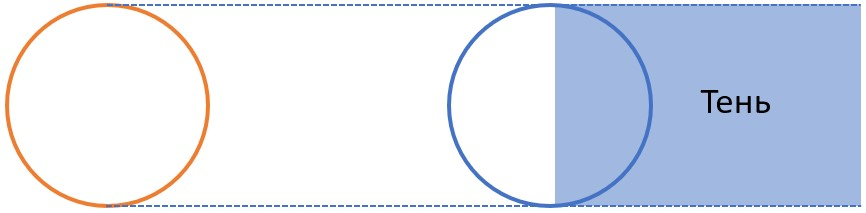
\includegraphics[width=\linewidth, height=6cm, keepaspectratio, valign=c]{review/cylindrical_shadow.jpg}
    \captionof{figure}{Цилиндрическая модель тени}
    \label{fig:cylindrical_shadow}
    
    \vspace{0.5cm} % Отступ между картинками
    
    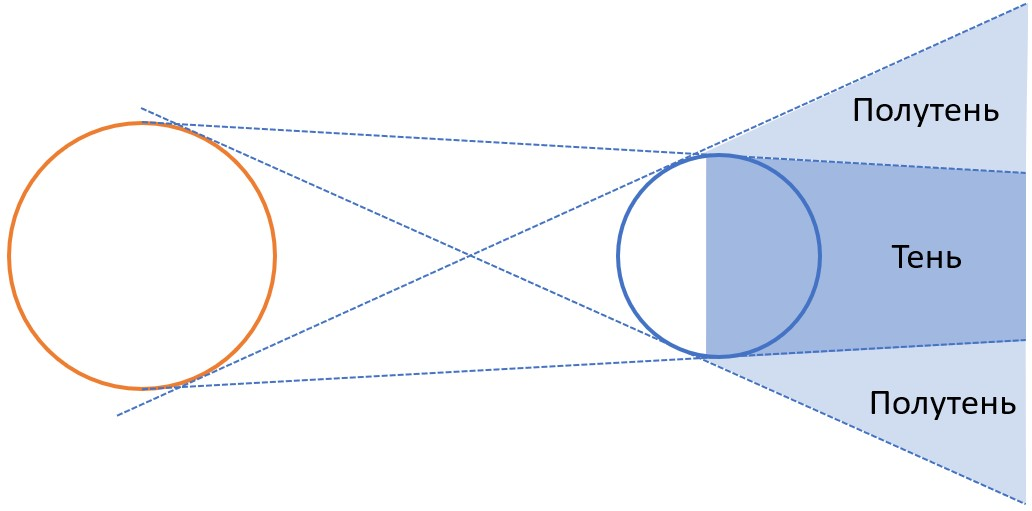
\includegraphics[width=\linewidth, height=6cm, keepaspectratio, valign=c]{review/conic_shadow.jpg}
    \captionof{figure}{Коническая модель тени}
    \label{fig:conic_shadow}
  \end{minipage}
  \hfill
  % Правый блок: 1 картинка по центру
  \begin{minipage}[c]{0.3\textwidth}
    \centering
    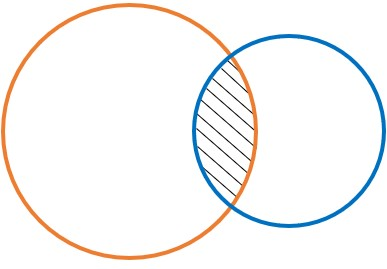
\includegraphics[width=\linewidth, height=6.5cm, keepaspectratio, valign=c]{review/area_shadow.jpg}
    \captionof{figure}{Модель тени с перекрытием}
    \label{fig:area_shadow}
  \end{minipage}

  \label{fig:combined}
\end{figure}

\paragraph{Альбедо} \mbox{} \\

Эффект альбедо связан с попаданием на спутник света, отраженного от Земли.
Значение отражательной способности сильно зависит от рода поверхности, на которую падает излучение.
Карта альбедо создается на основе спутниковых измерений, а поток изулчения,
воздействующий на спутник, рассчитывается для каждой части поверхности Земли отдельно и затем суммируется.

Поток энергии, падающий на КА в результате отражения от области площадью $dS$ на 
проверхности Земли, зависит от взаимной
ориентации КА и площадки, а также расстояния между ними:

\begin{equation*}
    J_{ds} = J_0 A \cos(\alpha) \cos (\beta) 
    \frac{dS}{|\mathbf{r}_{GCRS} - \mathbf{r}_{dS}|^2},
\end{equation*}
где $J_0$ -- падающий на площадку поток излучения от Солнца, 
$A$ -- энергетический коэффициент отражения (альбедо Земли),
$\alpha$ и $\beta$ -- углы падения и отражения луча, 
$\mathbf{r}_{GCRS}$ -- радиус-вектор КА,
$\mathbf{r}_{dS}$ -- радиус-вектор области (рисунок \ref{fig:albedo_geom}).

\begin{figure}[h!]
    \centering
    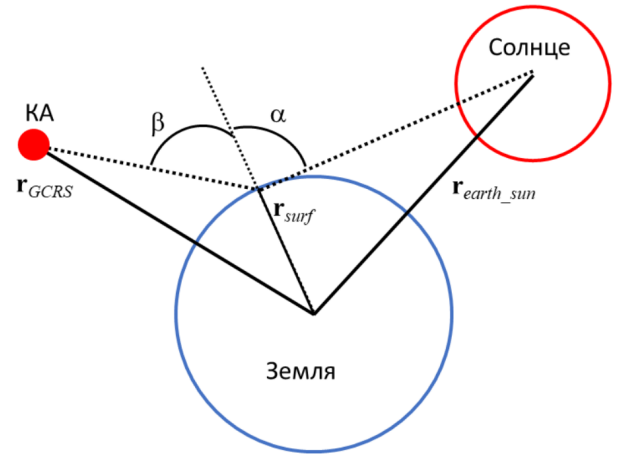
\includegraphics[width=0.7\linewidth]{review/albedo_geom.png}
    \captionof{figure}{Геометрия рассчета эффекта альбедо}
    \label{fig:albedo_geom}
\end{figure}

Альбедо Земли $A$ может быть вычислено по модели Кнока. В математической основе модели
разложение альбедо по зональным гармоникам:

\begin{equation*}
    A = a_0 + a_1 P_1 (\sin\phi) + a_2 P_2 (\sin \phi),
\end{equation*}
где $a_0, a_1, a_2$ -- параметры альбедо и излучения, причем $a_1$ и $a_2$ периодические по
времени, а $P_1$ и $P_2$ -- полиномы Лежандра первой и второй степени соответственно.

Сила давления отраженного излучения вычисляется из потока энергии, падающего на КА,
так же, как и при расчете силы солнечного давления.

% \begin{figure}[h!]
%     \centering
%     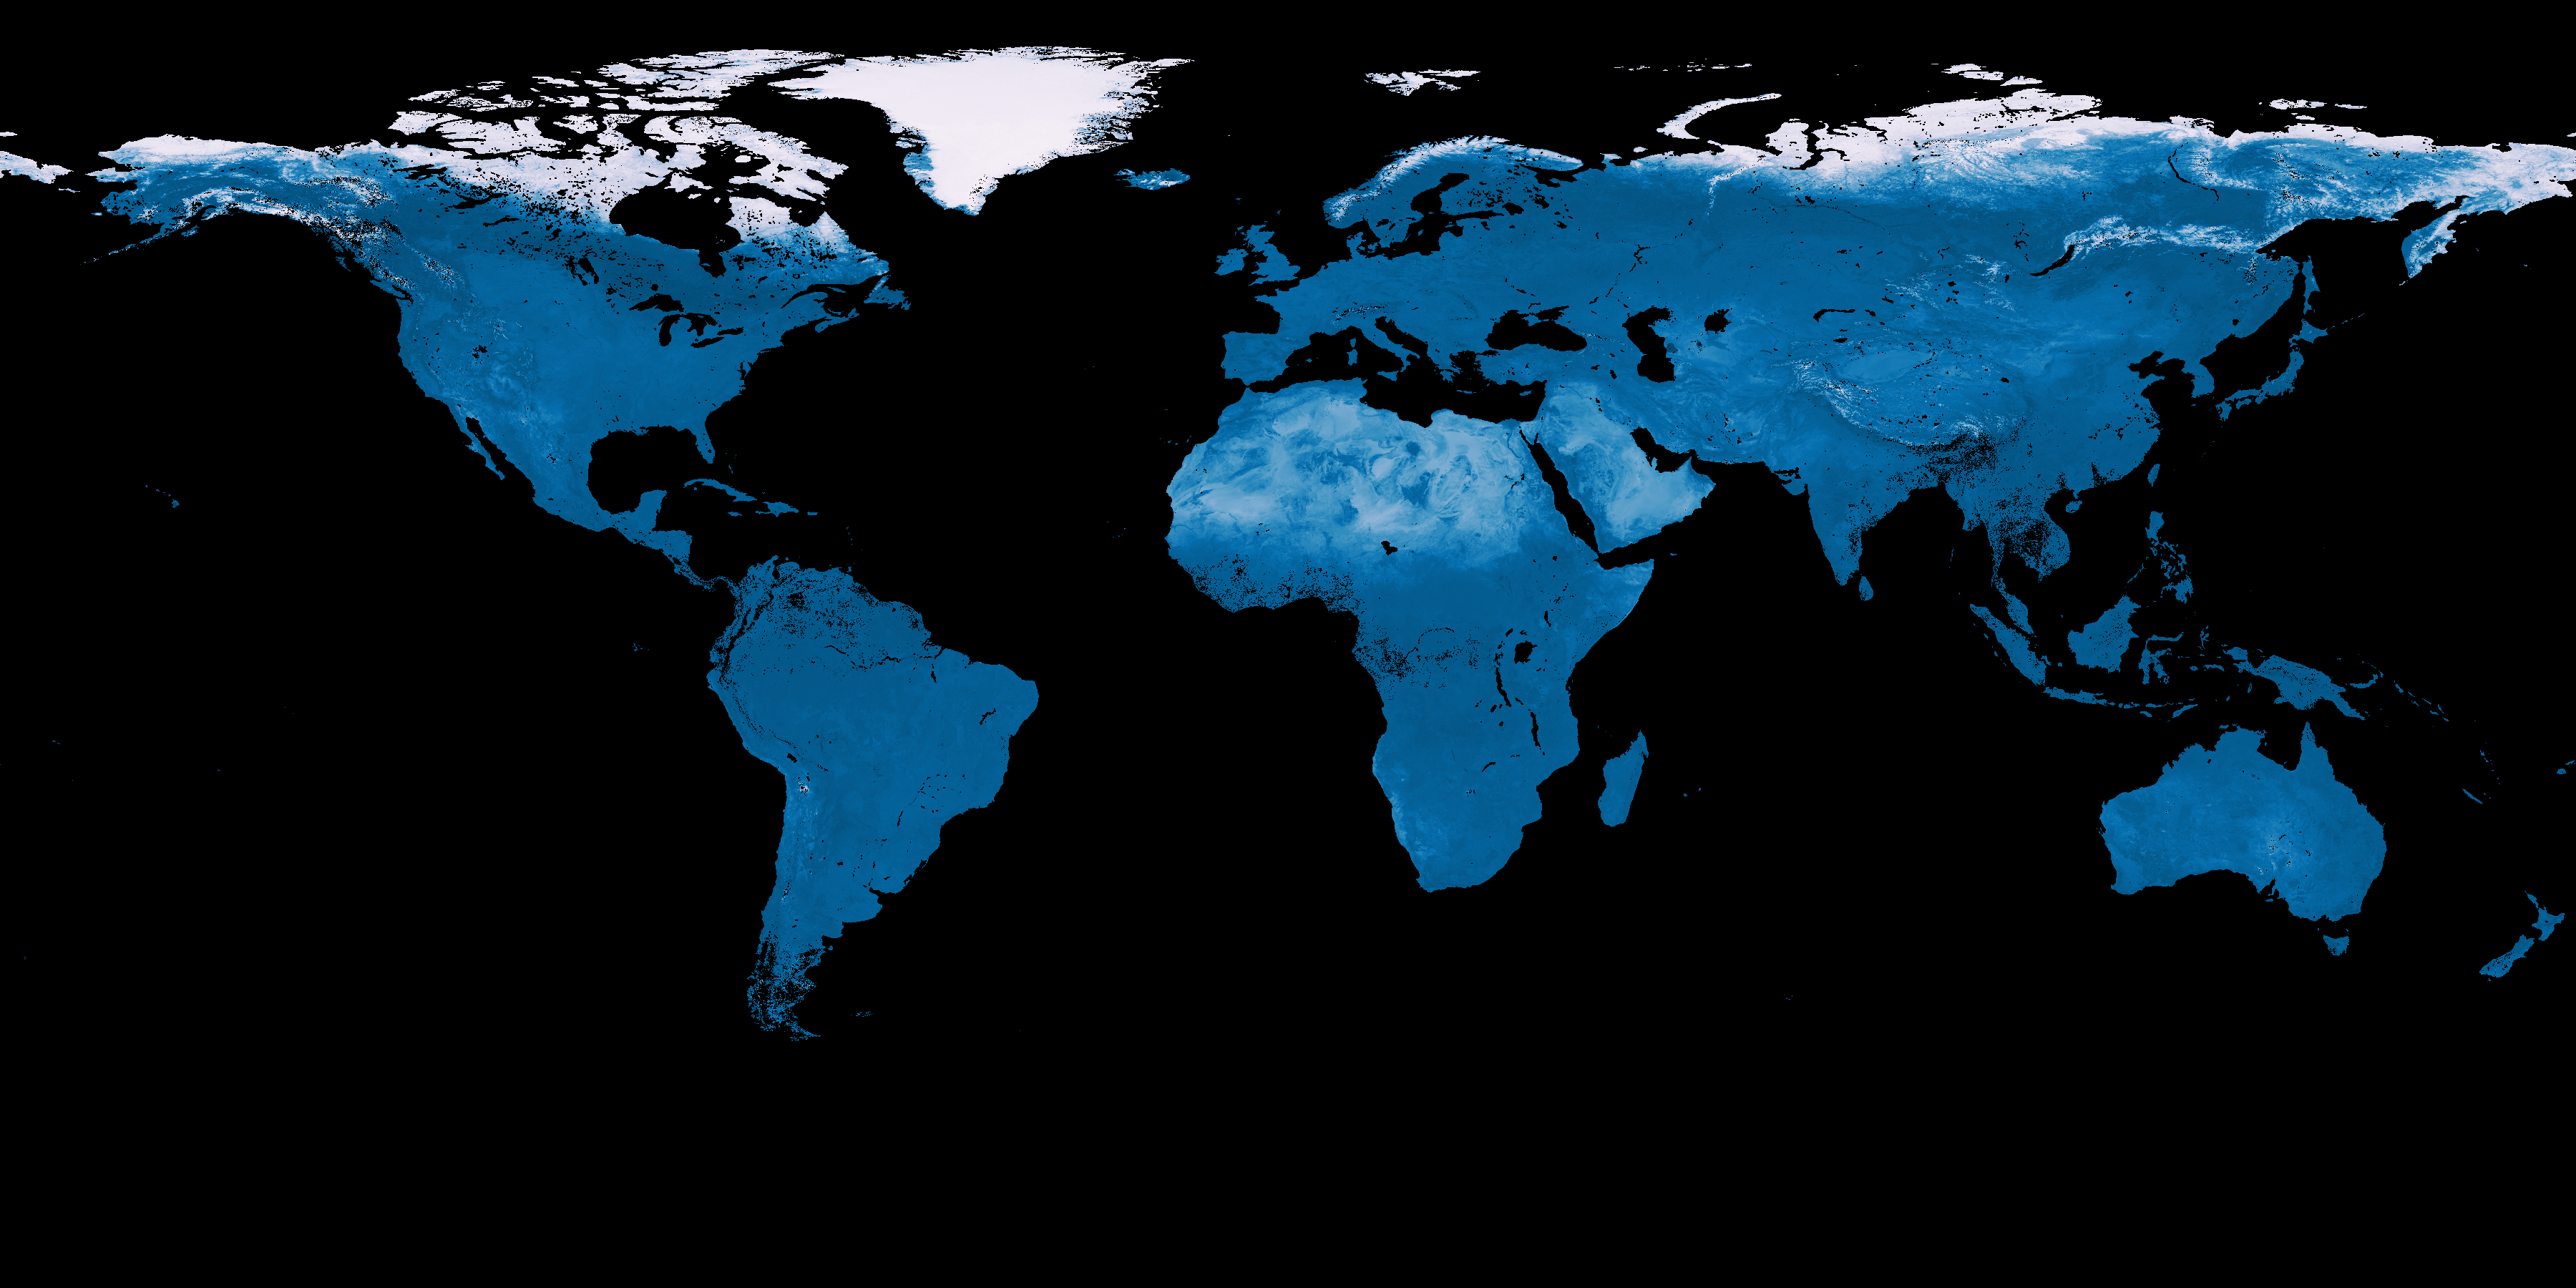
\includegraphics[width=\linewidth]{review/albedo_map.jpg}
%     \captionof{figure}{Карта альбедо, май 2025 г. Светлые участки
%     соответствуют областям с высокой отражательной способностью}
%     \label{fig:albedo_map}
% \end{figure}

\paragraph{Методы численного интегрирования} \mbox{} \\

Для интегрирования уравнений движения, то есть для решения задачи Коши вида \ref{eq:prognoz_task},
разработано групп методов. 

К первой группе относятся одношаговые методы, например,
семейство методов Рунге-Кутты (классический метод Рунге-Кутты, метод Дорманда-Принца).
В одношаговых методах состояние системы на следующем шаге вычисляется из комбинации
текущего состояния и его производных в промежуточные моменты времени. Данная группа
методов характеризуется простотой реализации,
однако явные одношаговые методы имеют существенные ограничения по точности и устойчивости.

Многошаговые методы (например, метод Гаусса-Джексона, методы Адамса), 
составляющие вторую группу, работают по схеме "предиктор--корректор".
Предиктор вычисляет прогноз на основе текущего состояния и производных в предшествующие
моменты времени, затем прогноз уточняется корректором. Сложность применения 
многошаговых методов заключается в необходимости дополнительных вычислений с использованием
других методов интегрирования для старта расчетов. Еще один недостаток подобных методов -- 
ограничение на порядок.

В неявных многошаговых методах можно достичь большей устойчивости и такого же порядка аппроксимации, 
как и в явных схемах, при меньшей стадийности. В задачах баллистики это означает сокращение количества 
подсчетов правой части и, следовательно, увеличение скорости работы. Высокая устойчивость
необходима в жестких задачах, например, при интегрировании высокоэллиптических орбит.

В качестве примера одношагового неявного коллокационного метода рассмотрим 
интегратор Эверхарта. В подходе Эверхарта правая часть интерполируется полиномом,
поэтому точность определяется выбором точек коллокации. Так, при выборе разбиения
Гаусса-Радо порядок аппроксимации равен $2 s - 1$, где $s$ -- стадийность метода.
Изначально метод Эверхарта создавался для построения траекторий комет, 
но в настоящее время он также широко используется в задачах прецизионного прогноза траектории.